\chapter{Implementation}

%The implementation should look at any issues you encountered as you tried to implement your design. During the work, you might have found that elements of your design were unnecessary or overly complex; perhaps third party libraries were available that simplified some of the functions that you intended to implement. If things were easier in some areas, then how did you adapt your project to take account of your findings?

%It is more likely that things were more complex than you first thought. In particular, were there any problems or difficulties that you found during implementation that you had to address? Did such problems simply delay you or were they more significant? 

%You can conclude this section by reviewing the end of the implementation stage against the planned requirements. 

\section{Database}
\textbf{NOTES: - DELETE THIS -}
\begin{itemize}
	\item Nodes and Ways downloaded from OpenStreetMap\cite{OSM}, and stored in a \textit{.osm} file. Size of downloadable area restricted.
	\item All data read by an XML-reader made by Vogella \cite{Vogella-XML}, and stored in two separate Arrays for Nodes and Ways (The type: Relations is not stored). Data filtered afterwards in order to reduce memory-requirements, and to speed up route-planning.
\end{itemize}

Using routing-data downloaded from OSM while the system is running proved to be much more challenging than first expected. Because paying for access to this data was out of the question, only free services remained as an option. But because these services are free, there are heavy restrictions put on how much data we are allowed to download at a time, and also restrictions put on the speed of the connection to the server. Without these restrictions, the servers would obviously be bogged down really quickly by the constant high demand for data from its users, so it is quite easy to understand why the restrictions were put in place. But because these services were so restricted, they proved to be unsuitable for the amount of tests run on this system during development -- which is a direct result of programming using Test Driven Development.
Another issue with downloading routing-data from a third-party, is that the functionality of the system is made dependent on several third parties like the routing-data-provider and user's ISP.
As mentioned a couple of times already: The author's internet-connection was not always reliable during the development of this system, so a decision was made to store routing- and map-data locally in an attempt to guard against further delays in development.

All routing-data is stored locally in a \textit{.osm} file downloaded directly from OpenStreetMap's website\cite{OSM}. This download was restricted to a relatively small area, so the Penglais campus of Aberystwyth University was chosen as the testing-grounds during development because it is (almost) small enough to fit inside the boundaries of the download (See Figure \ref{fig:badDataBadPath}), and because the author is very familiar with this area, erroneous routes were easy to spot.

It is possible to download routing-data covering much larger areas from other servers like Geofabrik\cite{geofabrik}, but these files are usually massive, and use a lot of memory when unzipped, so the \textit{.osm} file downloaded directly from OSM seems like a good compromise between space-complexity (when compared to Geofabrik), and time-complexity (when compared to downloading Nodes and Ways while the system is running).

The \textit{.osm} file is read by an XML-reader developed by Lars Vogel \cite{Vogella-XML}, and copied into separate arrays for Nodes and Ways. Connections between Ways (not to be confused with \textquotedblleft Relations\textquotedblright\cite{OSM-Relation}) are formed whenever two or more Ways reference the same Node, which is easy to detect because every Way links to specific Nodes in the array of Nodes, thus ensuring that they all reference the same data.

After all of the data has been copied from the \textit{.osm} file, it is run through three filters to remove various types of data. One filter removes Ways that are inaccessible to PRMs (eg. stairs, residential housing, or Ways marked explicitly as inaccessible), another filter removes Ways that are unrelated to pedestrian pathfinding (eg. forests, railings, or traffic signs), and the third filter removes inaccessible doors from buildings, as well as isolated Nodes and Ways. These filters reduce the amount of data stored by the system, as well as reduce the number of possible paths available for route-planning -- reducing run-times.

\begin{figure}
	\centering
	\caption[Sup-optimal path due to bad data]{This image shows what can happen to a route if the algorithms are working with bad data. The path between the start and goal positions is not included in the .osm-file, so the search-algorithms were forced to find a much longer route.}
	\label{fig:badDataBadPath}
	\frame{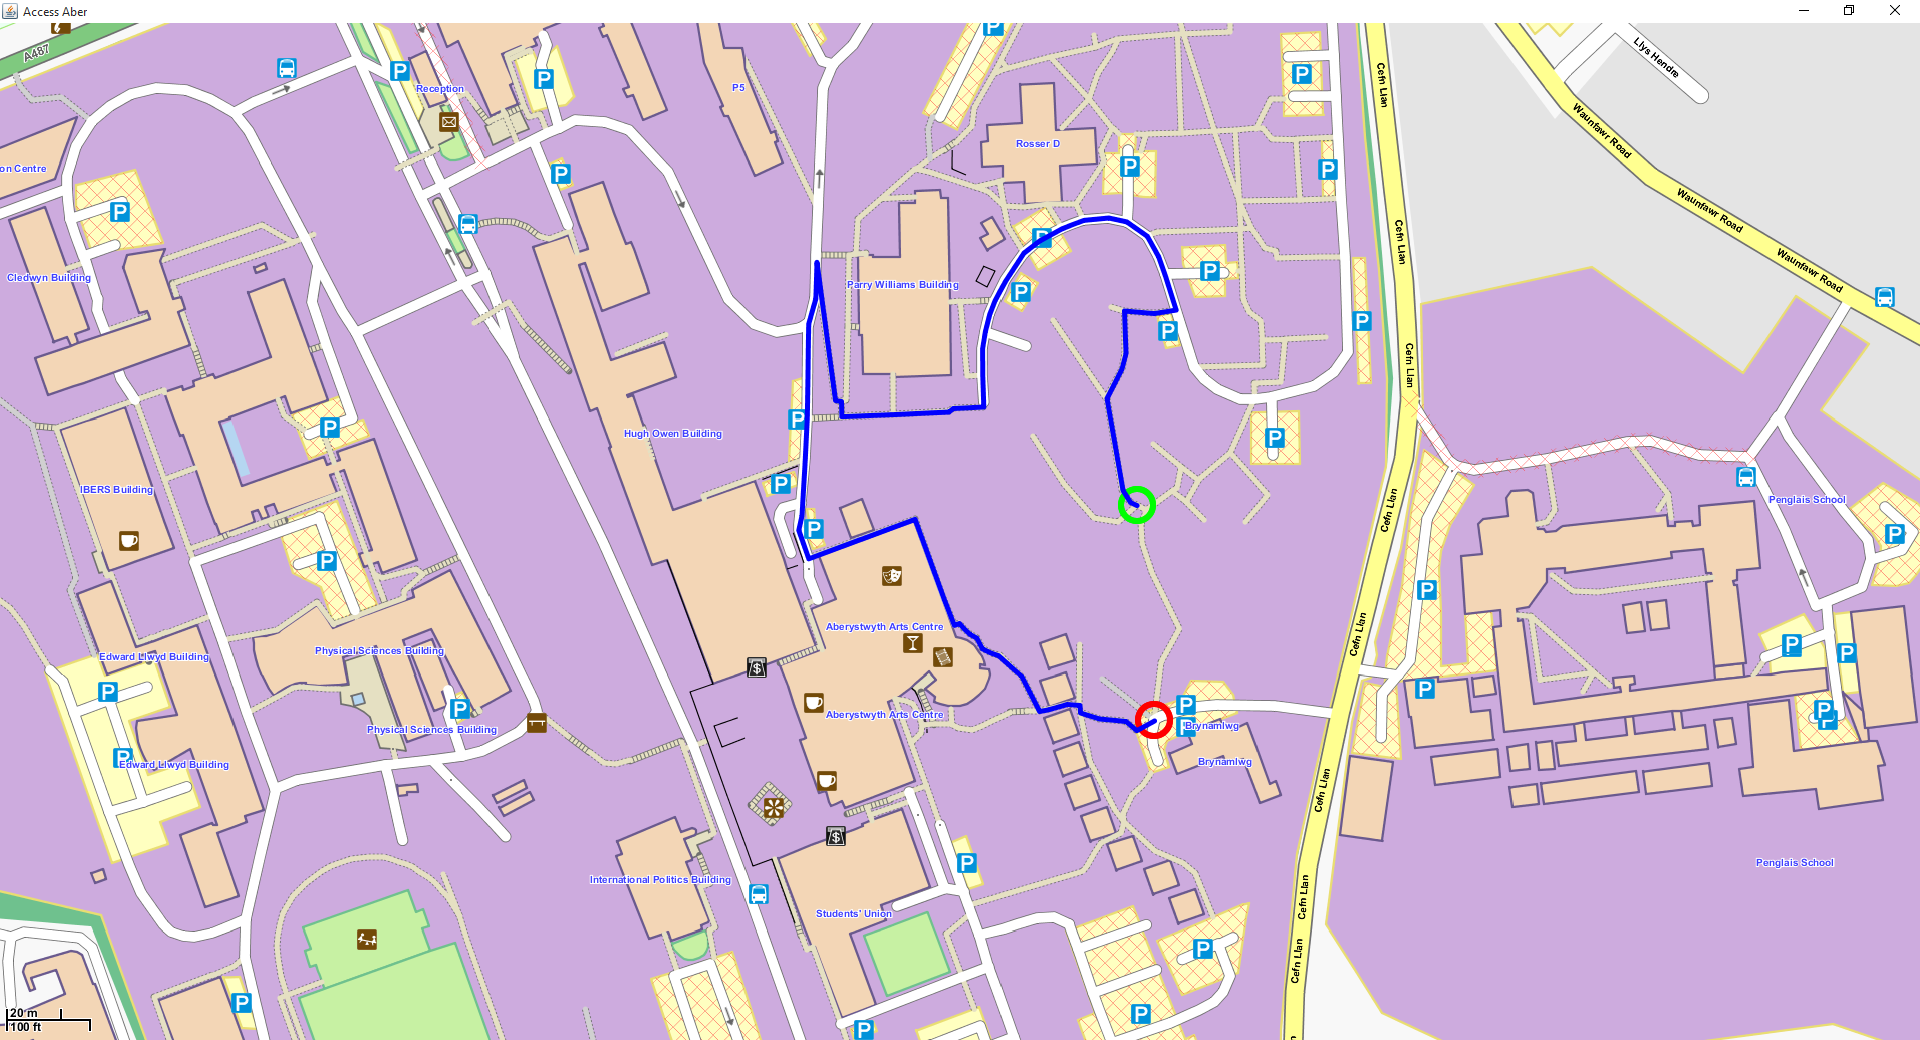
\includegraphics[keepaspectratio, width=\columnwidth]{Images/AStar_Missing_Node-data}}
\end{figure}

\section{Search}
\textbf{NOTES: - DELETE THIS -}
\begin{itemize}
	\item Is this where I describe my algorithms, or do I do that in chapter 2?
	\subitem I think I do it in chapter 2. This chapter should discuss any unexpected issues encountered during development.
	\item A Star, Breadth First Search, Depth First Search, Greedy Best First Search.
	\item PQ did not reorder after the values of its contents changed (after being sorted).
	\item PQ and expansion list not cleared between runs. Used old routes. (Touch on how this can be a good thing if done properly; time/space complexity).
	\item Only tower Nodes used for navigation. Very useful as some ways can have >100 Nodes, but far fewer connections to other Ways.
	\item Three enums: 'Permitted tags', 'Disallowed tags', and 'Area tags' dictate the way in which Nodes are expanded, discarded and handled afterwards.
	\item Include a table / graphic showing the difference in time- and space-complexity between the different algorithms.
	\subitem Should I do this in chapter 2 instead?
\end{itemize}

This route-planning system will always plan accessible routes, as any inaccessible Ways are removed as the routing-data is loaded, and before any routing-algorithms are run.

Runtimes and memory-requirements are reduced by only planning routes via Tower Nodes, and skipping Pillar Nodes altogether (except when calculating path-costs). This abstraction of routing-data into only a subset of path-connections is comparable to the systems described by Yang et al.\cite{CCAI07}, and Botea et al.\cite{botea-etal-jogd04}, with a few key differences.

This system groups Tower Nodes by the physical structures they represent, while most other hierarchical path-finding systems group Nodes by their geographical position, with respect to some artificial divide in the data. The latter form of hierarchical path-finding reduces the number of stored Node/Way-connections to an almost constant number of connections between areas, no matter how large the dataset becomes. My system will store at least two connections for each grouping (one entry and one exit point), and the number of total connections stored will therefore increase with the number of Ways in the routing-data. This means that other hierarchical path-finding systems scale much better than my system when given increasing amounts of routing-data, but as already discussed: Those systems sometimes find somewhat sub-optimal paths, whereas my system always finds truly optimal paths (provided that an optimal search-algorithm is employed).

A quite big issue encountered during development, was the way Java's priorityQueue-library handled an item's weights being updated after it had been added to the queue. If an item is in the priorityQueue, then its position will not change even if its weights do -- unless it is removed and then added again. This means that A* in particular was unable to reorder its expansion-queue when a better path-cost to an already expanded Node was found, which occurs quite often in A*, and is a key part of how it finds optimal paths.

This problem was solved by first removing and then adding the Node to the priorityQueue again, but this could -- in the worst case -- result in iterating to the last position in the queue twice ($O(2n)$) if that Node's path-cost is worse than that of any other Node in the queue before and after being updated.

My system is not able to reuse old routes when planning new ones, which would be a very beneficial, and time+memory saving feature on longer routes. Because the user is only able to move either the start or goal-marker before a new route is planned, the new route could be planned from whichever marker was moved to the other marker, or alternatively a Node in the old route. If the new route enters the old route, then we know that there cannot be a better path to/from the Node it is connected to, so the rest of the new path can safely reuse the remainder of the old path to the marker that was not moved.

The issue with this type of reuse is that it assumes that the path-cost going in one direction is the same as the cost of going in the opposite direction, which is not true when considering the inclination of a path. The inclination of roads is not currently considered by the system when planning routes, but because this was a planned feature, there was no reason to consider reusing old routes\footnote{If the start-marker is moved, then the old optimal path to the goal-marker can be reused if it is found, but this is not true if the goal-marker is moved.}.

\begin{figure}
	\centering
	\caption{Algorithms avoid stairs}
	\label{fig:avoidStairs}
	\frame{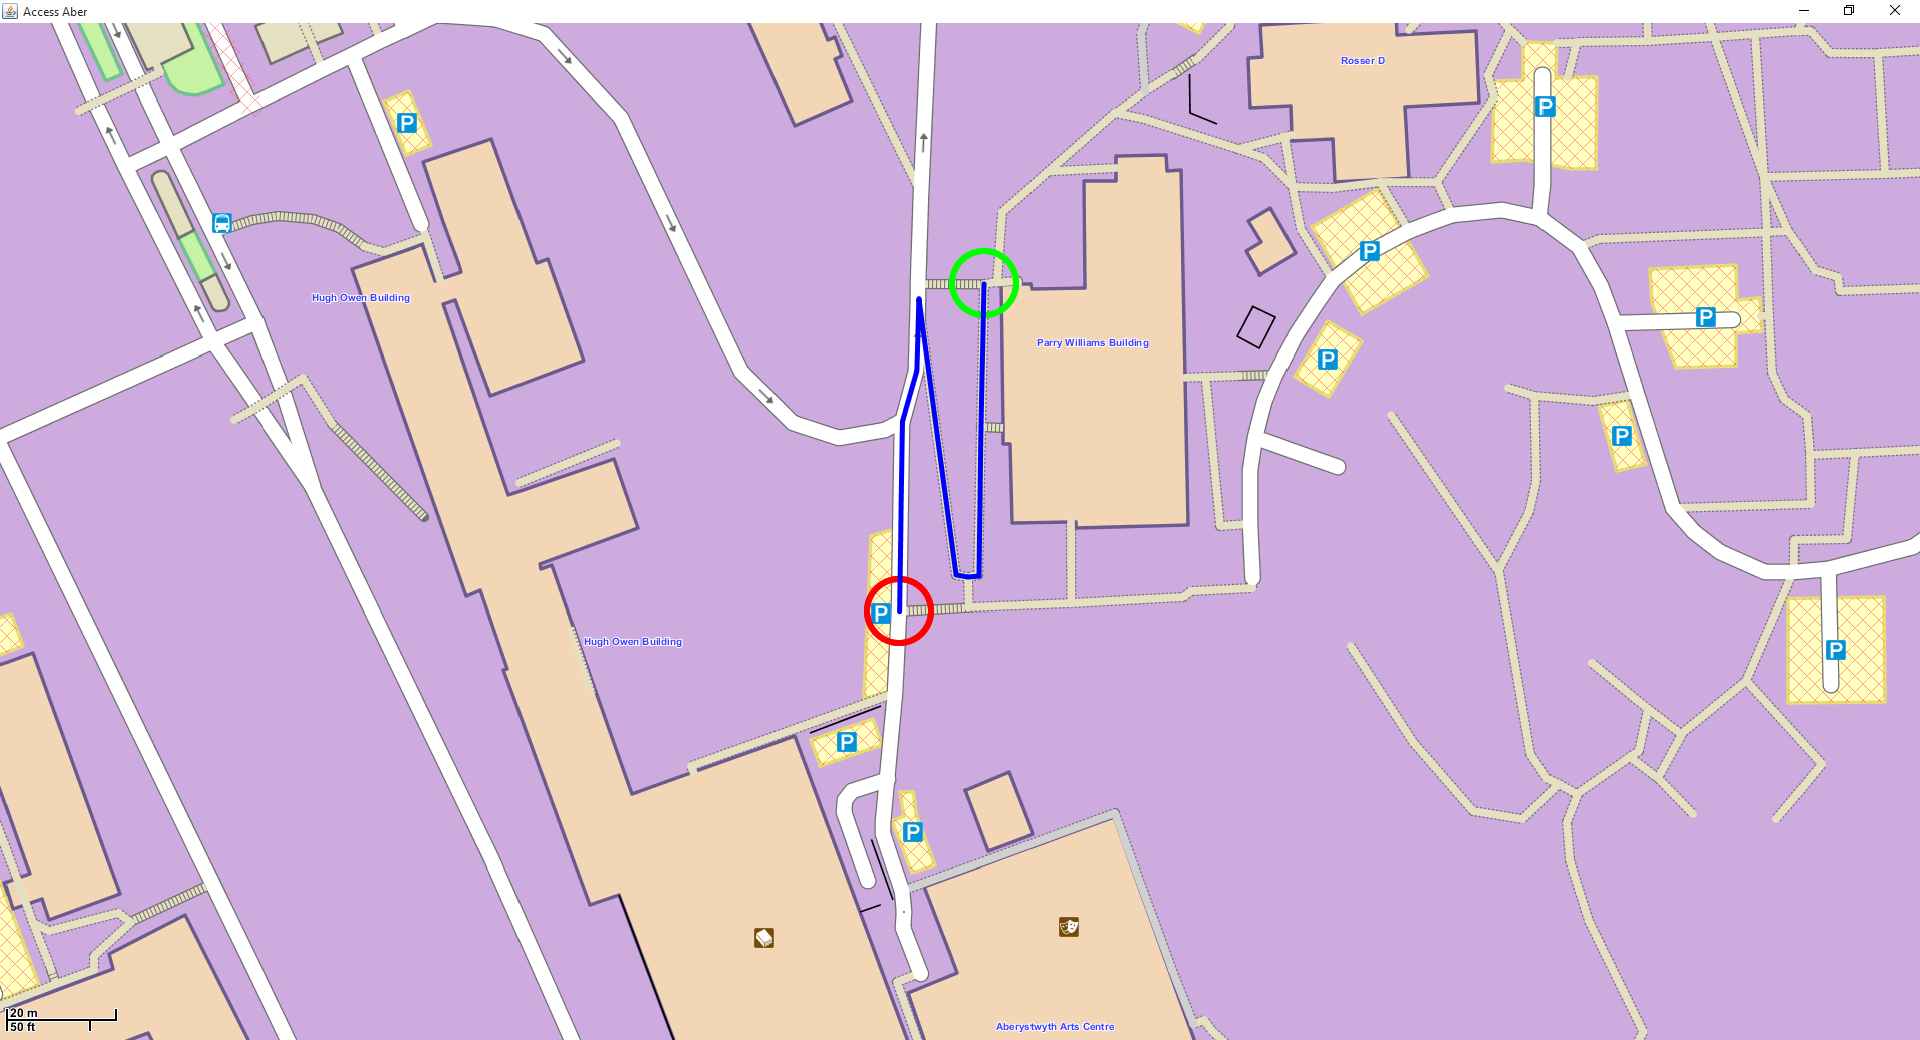
\includegraphics[keepaspectratio, width=\columnwidth]{Images/AStar_Avoids_stairs}}
\end{figure}
\begin{figure}
	\centering
	\caption{Algorithms avoid stairs 2}
	\label{fig:avoidStairs2}
	\frame{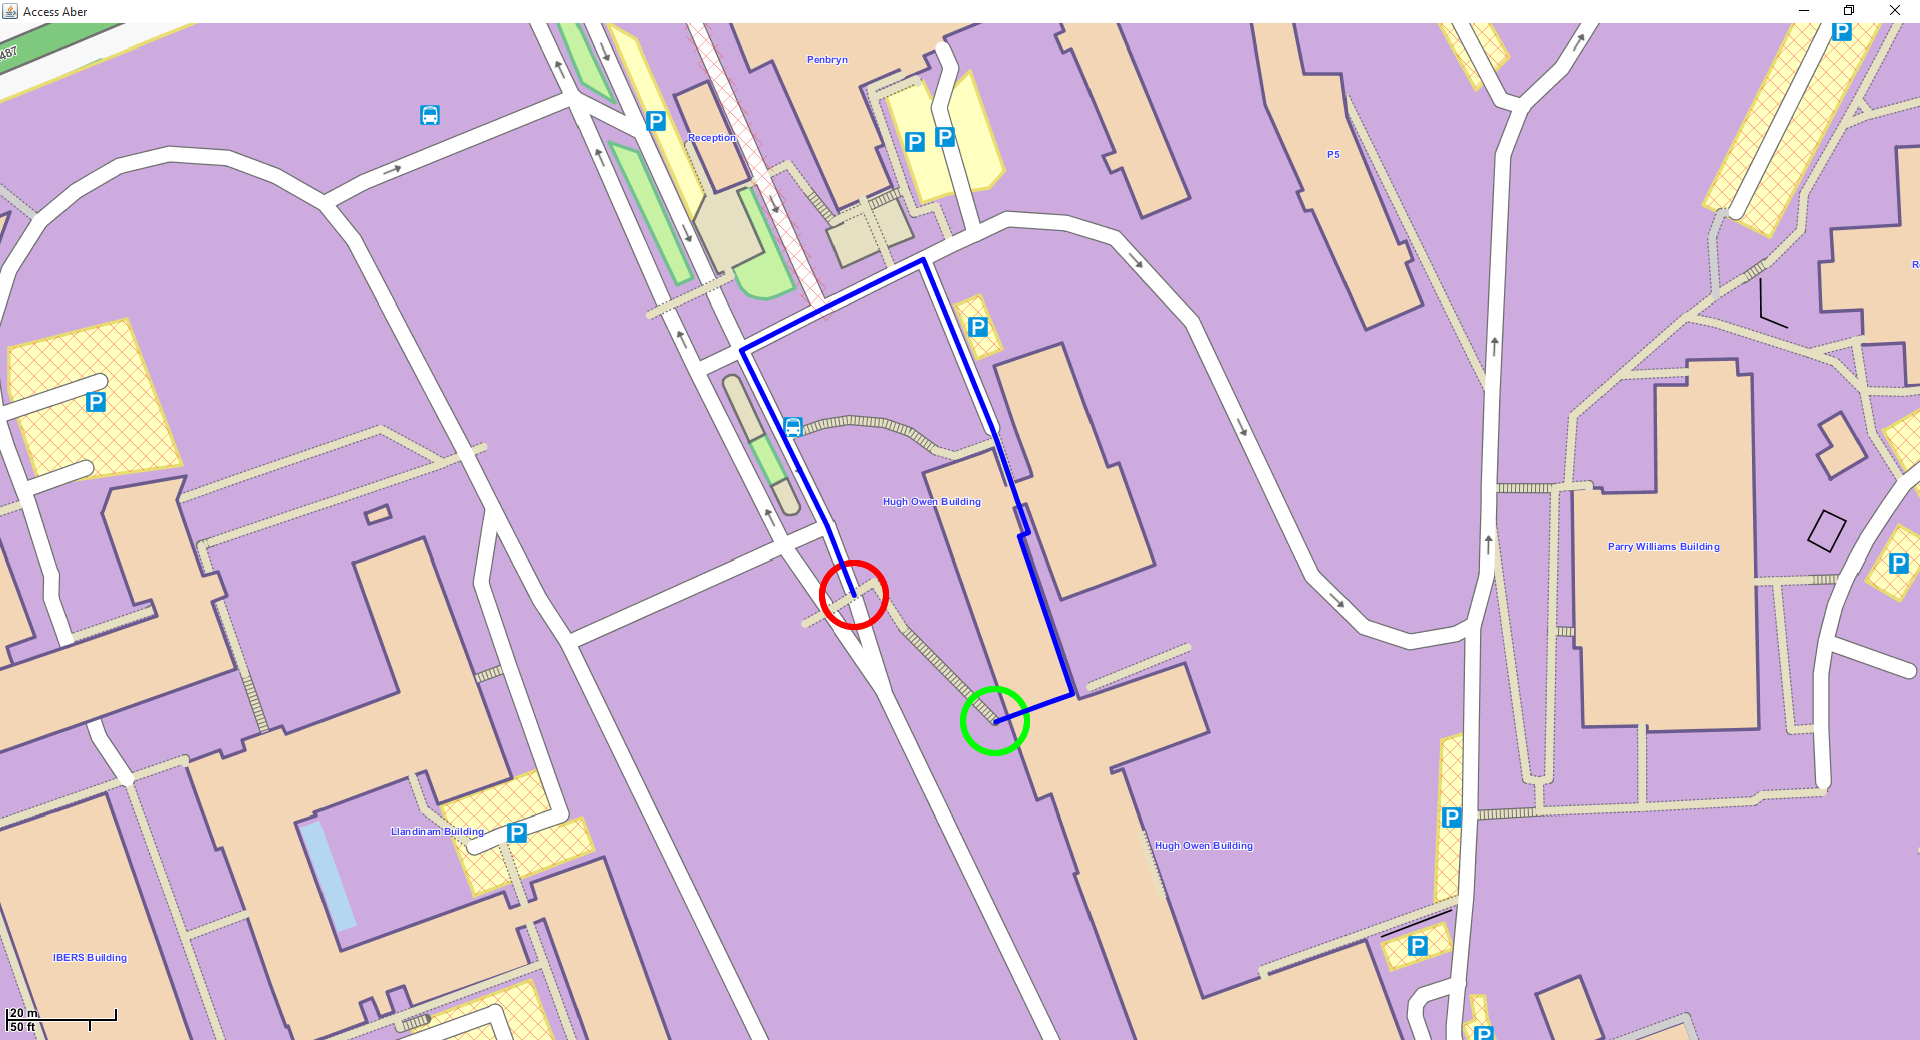
\includegraphics[keepaspectratio, width=\columnwidth]{Images/AStar_Avoids_stairs2}}
\end{figure}

\section{Map}
\textbf{NOTES: - DELETE THIS -}
\begin{itemize}
	\item Map-API from Mapsforge \cite{Mapsforge}. GraphHopper considered -- they also use Mapsforge.
	\item Compare routes from Google Maps, GraphHopper(OSM), and Mapzen(OSM) to my system's routes? IMPACS to SU? Screenshots?
	\item show how the routes were drawn straight across lawns when Pillar Nodes were ignored (sent an example of this in an email to Myra).
\end{itemize}

The map used in this system has been provided by Mapsforge\cite{Mapsforge,Mapsforge_map-tiles}. Both the map-tiles and classes and methods used to display them come from Mapsforge.
The map-tiles are stored locally, as opposed to being downloaded whenever a route is planned in an area, because it takes some time to download this data without a dedicated server. A couple of free map-tile providers were tested during the development of this system, but as they all restricted download-speeds quite heavily, displaying the map took a little too long, not to mention zooming or moving the map-view around.

The map-tiles stored locally cover the entirety of Wales, Great Britain, while the routing-data stored i the \textit{.osm} file only covers the Penglais campus of Aberystwyth University, so these map-tiles are more than good enough to display every possible route planned by the system.

In order to plan a route, you can either input five commands as arguments to the system before running it ((text)algorithm, (decimal number)latitude1, (decimal number)longitude1, (decimal number)latitude2, (decimal number)longitude2), or alternatively start it without any input-commands. If the system is started without any input-arguments, it chooses A* as the default routing-algorithm, and waits for the user to click on two separate locations before it plans a route between them. After a route has been planned and displayed to the user, they can click anywhere else on the map, and the start- or goal-Node will be moved to that location depending on which is closer.


\section{Fulfilment of requirements}
\textbf{NOTES: - DELETE THIS -}
\begin{itemize}
	\item Storage of OSM-data in separate Arrays for Nodes and Ways.
	\item OpenStreetMap database not updated with new and/or more accurate information.
	\item Good routing-algorithm found; A* guarantees optimality and completeness. Other algorithms are able to use less memory and find routes faster, but A* works fine on a small area like the Penglais campus of Aberystwyth University.
	\item Created filters able to easily exclude many Nodes/Ways from the search. Very easy to add and remove labels in the filters. Filters made for wheelchair-users only.
	\item No localisation (eg. GPS) implemented, but added functionality to find the Node closest to some coordinates and set it as the start/goal position, thus making it relatively easy to use localisation to set the user's position in the future. The coordinates need to use the same coordinate-system as the OSM-data though.
\end{itemize}

\begin{enumerate}
	\item Make it clear that PRMs need to be considered by more route-planners
	\subitem This project has uncovered routes that may be fine for able-bodied pedestrians, but are completely inaccessible for PRMs; See Figure \ref{fig:longerRoutePRM}, where an able-bodied pedestrian would be able to walk in an almost straight line up the stairs to the Student Union, a PRM would need to take several detours.
	\item Distinguish between accessible and inaccessible routes
	\subitem Three filters have been created to remove inaccessible and irrelevant data. The system is also able to plan routes through buildings, finding much shorter and practical routes for PRMs than most other conventional route-planning systems are able to.
	\subitem It should be very easy to add and remove labels in the filters, making sure that keeping the system up-to-date is relatively painless. The filters are only made for wheelchair-users though, except for the Building/Area-filter which can be a useful addition to any route-planner for pedestrians.
	\item Find optimal and complete algorithm(s)
	\subitem A* is optimal and complete, and paired with the fact that the routing-data is abstracted by only using Tower Nodes for route-planning, the algorithm and system as a whole get many of the same benefits presented by a hierarchical path-finder.
	\subsubitem This implementation of A* is still much slower than other hierarchical path-finding-algorithms when used to plan longer routes however, and works best on smaller areas. Most PRMs are unlikely to travel great distances though, at least on foot or in a wheelchair -- which are the methods of locomotion that this route-planner is made for.
	\item Algorithm(s) have to plan routes in near-real-time, and use as little memory as possible.
	\subitem The routing-data is filtered to only contain information relevant to routing, and paths are sped up by only using Tower Nodes while routing -- making it possible to jump from one Way to another in a single Node-expansion. All of this reduces the time- and space-complexity of the system.
	\item Display the routes on a map
	\subitem Mapsforge\cite{Mapsforge,Mapsforge_map-tiles} displays the map, using map-tiles stored locally on the system.
	\item No localisation (eg. GPS) implemented, but added functionality to find the Node closest to some coordinates and set it as the start/goal position, thus making it relatively easy to use localisation to set the user's position in the future. The coordinates need to be in the same coordinate-system as OSM's routing-data though\cite{OSM_Convert-WGS84}.
\end{enumerate}